% SNAS 2026 double-blind short-paper submission candidate.
% Compile with XeLaTeX so the document uses Times New Roman.
\documentclass[12pt,letterpaper,twoside]{article}

\usepackage[margin=1in]{geometry}
\usepackage{fontspec}
\setmainfont{Times New Roman}
\usepackage{setspace}
\doublespacing
\usepackage{booktabs}
\usepackage{graphicx}
\usepackage{caption}
\usepackage{fancyhdr}
\usepackage{titlesec}
\usepackage{xurl}
\urlstyle{same}
\usepackage[hidelinks]{hyperref}
\hypersetup{
  pdftitle={ConstructionSafety-FaithBench: Auditing Visual-Evidence Faithfulness in Construction-Safety Vision-Language Models},
  pdfauthor={},
  pdfsubject={Double-blind short-paper submission candidate},
  pdfkeywords={trustworthy AI, explainable AI, vision-language models, construction safety, evidence faithfulness}
}

\setlength{\parindent}{0.5in}
\setlength{\parskip}{0pt}
\setlength{\emergencystretch}{3em}
\setlength{\textfloatsep}{8pt plus 2pt minus 2pt}
\setlength{\floatsep}{6pt plus 2pt minus 2pt}
\captionsetup{font=small,skip=3pt}
\raggedbottom

\titleformat{\section}
  {\normalfont\bfseries\centering}
  {\thesection.}{0.5em}{}
\titlespacing*{\section}{0pt}{8pt}{4pt}
\titleformat{\subsection}
  {\normalfont\bfseries}
  {\thesubsection.}{0.5em}{}
\titlespacing*{\subsection}{0pt}{6pt}{2pt}

\pagestyle{fancy}
\fancyhf{}
\fancyhead[LE,LO]{\textit{ConstructionSafety-FaithBench}}
\fancyhead[RE,RO]{\thepage}
\renewcommand{\headrulewidth}{0.4pt}
\setlength{\headheight}{15pt}

\newenvironment{apareferences}
  {\begin{list}{}{%
    \setlength{\leftmargin}{0.5in}%
    \setlength{\itemindent}{-0.5in}%
    \setlength{\itemsep}{0pt}%
    \setlength{\parsep}{0pt}%
    \setlength{\topsep}{0pt}}}
  {\end{list}}

\begin{document}

\begin{center}
\textbf{ConstructionSafety-FaithBench: Auditing Visual-Evidence Faithfulness in Construction-Safety Vision-Language Models}
\end{center}

\begin{center}
\textbf{Abstract}
\end{center}

Construction-safety vision-language models (VLMs) can produce the right safety answer for the wrong visual reason. A model may classify a scene as unsafe because construction context looks hazardous, while ignoring the specific worker, protective equipment, edge, or machine-proximity cue that the safety rule actually depends on. We introduce ConstructionSafety-FaithBench to audit this right-answer/wrong-evidence gap. The benchmark separates three questions that are usually merged: whether the answer is correct, whether the cited visual evidence is rule-relevant, and whether the answer changes when that evidence is removed. We evaluate automated baseline annotations and a Florence-2 grounding adapter on hard-hat, fall-protection, guardrail, and struck-by rules, then apply targeted occlusions to rule-relevant boxes and compare them with same-size random masks. On a prioritized audit set where Florence-2 often disagrees with the automated baseline, Florence reaches 18.3\% accuracy and 12.5\% macro-F1, while the baseline reaches 78.3\% accuracy. More importantly, masking rule-relevant evidence changes Florence answers 39.2\% of the time, compared with 9.2\% for matched random masks. The result indicates that safety judgments can depend on specific local pixels, so answer scoring alone cannot establish visual-evidence faithfulness.

\noindent\textit{Keywords:} trustworthy AI; explainable AI; vision-language models; construction safety; evidence faithfulness; AI risk assessment

\section{Introduction}

Construction sites are dynamic environments where safety status depends on small, localized, rule-specific visual cues: a hard hat on a worker, a guardrail at an exposed edge, a harness at height, or equipment near a pedestrian path. Vision-language models are attractive for screening such imagery because they can combine natural-language rules with visual inputs. At the same time, they behave like black-box safety assistants: they may return fluent answers without exposing whether those answers come from the relevant visual evidence.

This creates an explainability gap. White-box inspection is rarely available for deployed VLM systems, so safety evaluation needs practical perturbation-based tests. We operationalize two requirements from explainable safety review: descriptive accuracy, where the cited evidence should match the rule-relevant cue, and robustness, where behavior should change predictably when that cue is removed. In this paper, intervention sensitivity means a simple counterfactual check: mask the worker's hard hat, harness, edge barrier, or equipment-proximity region, rerun the model, and test whether the answer or evidence changes more than it does under a same-size random mask. If the answer is correct but the evidence is irrelevant, the model may be relying on scene priors. If the answer is stable when rule-relevant evidence is removed, the model may not be using the visual cue it claims to use.

We address this gap with ConstructionSafety-FaithBench, a reproducible audit pipeline for visual-evidence faithfulness in construction-safety VLMs. Each example pairs a construction-site image with a natural-language safety rule, answer label, evidence regions, and provenance fields. The benchmark focuses on four rule families: hard-hat/PPE compliance, harness/fall protection, guardrail/edge protection, and struck-by/equipment proximity. The pipeline produces normalized manifests, model outputs, audit labels, intervention specifications, score tables, figures, and release manifests.

The study evaluates deterministic baselines and a Florence-2 grounding adapter, then tests whether targeted rule-evidence masks affect model behavior more than same-size matched-random masks. The results show why evidence-level auditing matters: Florence performs poorly on the prioritized audit set, and targeted occlusion produces substantially larger answer changes than random masking. The paper contributes a compact benchmark structure, a final audit-label layer with explicit provenance, and an intervention analysis that separates answer correctness from evidence dependence.

\section{Benchmark and Audit Pipeline}

Each row contains an image identifier, source split, natural-language safety question, normalized rule identifier, answer label, evidence boxes, and provenance metadata. Raw images and model weights are not redistributed; reproducible scripts load source images only when local dataset access is available.

Figure~\ref{fig:pipeline} summarizes the architecture. ConstructionSite-derived metadata and images are converted into pilot and scale-up manifests. Automated baseline annotations are generated from dataset metadata, captions, rule-violation records, and available boxes. Model adapters then write normalized CSV/JSONL outputs, and the scorer compares model answers with either the automated baseline annotations or the final audit labels. Intervention specifications reuse evidence boxes to compare targeted rule-evidence masks with same-size matched-random masks.

\begin{figure}[t]
\centering
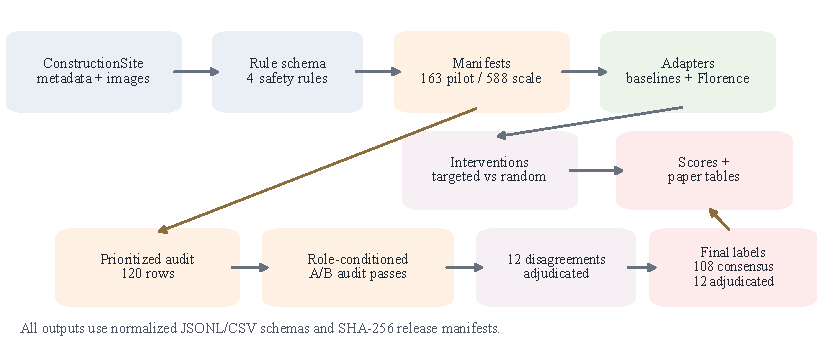
\includegraphics[width=0.88\linewidth]{figures/pipeline_architecture.pdf}
\caption{Benchmark architecture. The same schema supports manifests, model outputs, audit labels, interventions, score tables, and release manifests.}
\label{fig:pipeline}
\end{figure}

The audit stack has three layers. First, automated baseline annotations support scaling and triage, but they are not ground truth. Second, the prioritized audit set isolates difficult cases where Florence-2 and the automated baseline disagree or show weak evidence overlap; 118 of the 120 audited rows are Florence/baseline answer disagreements. Third, the final audit-label layer resolves these cases using two independent audit passes plus returned adjudication for disagreements. Final labels are reported with this provenance rather than as unqualified human ground truth.

\section{Metrics and Experimental Setup}

The benchmark reports three metric families. Answer metrics include accuracy and macro-F1 across compliant, violation, and uncertain labels. Evidence metrics include whether a model returns any evidence box, best overlap with the reference box, normalized centroid drift, and evidence disappearance after masking. Intervention metrics compare a targeted mask over rule-relevant evidence against five same-size random masks sampled per image. The paired statistic is the targeted effect minus the within-image matched-random mean.

The implemented adapters are intentionally simple and auditable. The automated baseline echoes the metadata-assisted label. Manifest seed and majority-violation baselines test weak-label and class-prior behavior. A caption-keyword baseline checks whether captions alone leak the labels. The Florence grounding adapter runs \textit{microsoft/Florence-2-base-ft}, prompts for rule-relevant objects, and maps grounded detections through deterministic geometry. Each adapter records normalized outputs and provenance.

Targeted occlusions are selected from the evidence boxes in the pilot manifest: for a hard-hat row this may be the worker/head region, for guardrails the exposed edge or barrier region, for fall protection the worker-at-height region, and for struck-by risk the worker/equipment proximity region. The targeted mask covers that rule-relevant box. The matched-random controls use the same clipped width and height but are placed elsewhere with low overlap with the target. The intervention study contains 948 Florence reruns: 158 targeted occlusions and 790 matched-random controls. Resampling intervals and paired tests are computed at the image level.

\section{Results}

Figure~\ref{fig:audit} shows the completed audit layer and answer scores. The final labels expose a sharp gap between automated annotation agreement and visually grounded model behavior. The automated baseline reaches 78.3\% accuracy against final labels because it is derived from the same metadata signals used to construct much of the candidate split. Florence grounding reaches only 18.3\% accuracy and 12.5\% macro-F1 on the prioritized audit set, which means the open-vocabulary grounding adapter often selects the wrong rule outcome even when it returns a plausible box.

\begin{figure}[t]
\centering
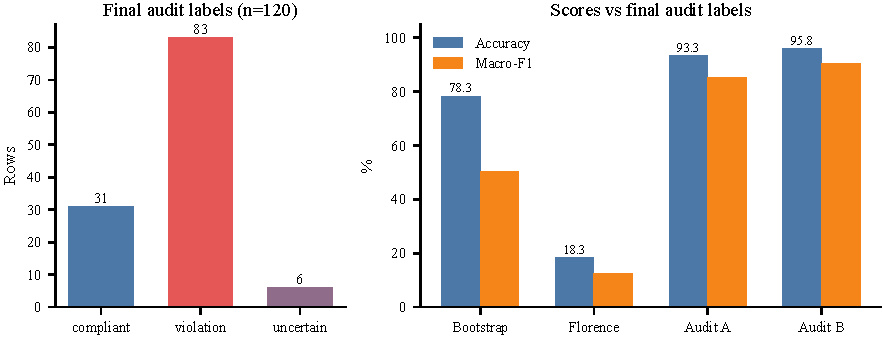
\includegraphics[width=\linewidth]{figures/audit_result_dashboard.pdf}
\caption{Final audit labels and answer scores. The audit split intentionally over-samples difficult disagreement and weak-overlap cases.}
\label{fig:audit}
\end{figure}

\begin{table}[h]
\centering
\caption{Headline results from the current audit and intervention study.}
\label{tab:headline}
\begin{tabular}{lr}
\toprule
Quantity & Value \\
\midrule
Final audit rows & 120 \\
Final audit label counts & 83 V / 31 C / 6 U \\
A/B agreement rows & 108 \\
Returned adjudication rows & 12 \\
Florence accuracy on final audit labels & 18.3\% \\
Automated baseline accuracy on final audit labels & 78.3\% \\
Targeted answer-flip rate & 39.2\% \\
Matched-random answer-flip rate & 9.2\% \\
Paired answer-flip difference & 30.0 points \\
Paired centroid-drift difference & 0.160 \\
\bottomrule
\end{tabular}
\end{table}

Figure~\ref{fig:intervention} summarizes the counterfactual faithfulness result. Targeted rule-evidence occlusion flips Florence answers 39.2\% of the time, compared with 9.2\% for same-size random masks. The paired answer-flip gap is 30.0 percentage points with a resampled 95\% interval of 22.3 to 37.7 points. This gap means the model is not responding only to broad construction-scene context; many predictions depend on local pixels associated with workers, PPE, edges, or equipment. However, it also shows fragility: removing the rule-relevant evidence often changes the answer rather than producing a calibrated ``uncertain'' response. Targeted masks also produce larger evidence relocation, with a paired centroid-drift difference of 0.160 and a 95\% interval of 0.133 to 0.187.

\begin{figure}[t]
\centering
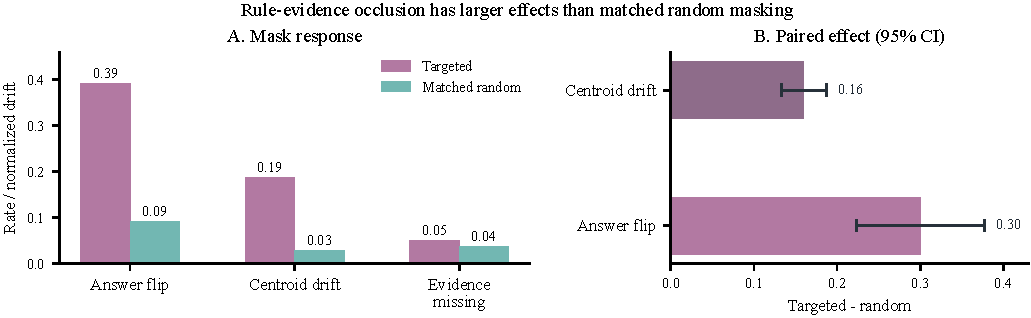
\includegraphics[width=\linewidth]{figures/intervention_effects_chart.pdf}
\caption{Targeted rule-evidence masking affects answers and evidence more than same-size random masking.}
\label{fig:intervention}
\end{figure}

The qualitative audit rows make the statistics concrete. In one PPE example, the adjudicated label is a violation because a third pedestrian in dark-green clothing is bare-headed while other workers wear yellow hard hats; a model that attends only to the visible helmets can miss the violation. In a fall-protection example, workers on elevated formwork lack a visible harness or lanyard, so the relevant evidence is the small worker-at-height region rather than the surrounding construction scene. In a struck-by example, a worker in high-visibility clothing stands near an excavator while it digs; the adjudication is compliant but ambiguous because the static frame cannot fully confirm distance or swing state. In guardrail examples, the difference between a walkable graded slope and an exposed edge changes the label. These cases show why construction-safety VLMs need rule-specific visual evidence rather than generic construction-site priors.

The scale-up results add a diagnostic pattern. Florence often returns some evidence region, yet answer accuracy remains weak and rule-dependent. Evidence presence is therefore not enough: a model can emit boxes while still using the wrong safety cue or producing the wrong answer.

\section{Discussion and Implications}

The main algorithmic finding is that answer correctness, visual evidence, and counterfactual sensitivity must be evaluated separately. Florence-2 is useful in this study because it exposes the limits of open-vocabulary grounding for construction safety: it can return boxes for objects such as workers, helmets, barriers, or equipment, but the mapping from those detections to a safety-rule judgment is brittle. A correct box is not always a correct rule interpretation, and a correct answer is not always supported by the right box.

The intervention analysis adds a second finding. The 30-point targeted-minus-random answer-flip gap suggests location-specific dependence: Florence is more sensitive to rule-relevant pixels than to arbitrary regions of the same size. But this is not the same as faithful reasoning. A robust safety assistant should change its answer for the right reason, preserve uncertainty when evidence is removed, and avoid replacing missing evidence with a confident guess. The benchmark can therefore support model comparison, regression testing, and audit documentation, but it cannot justify autonomous inspection, worker discipline, or surveillance.

\section{Limitations and Ethics}

The current study is not a deployment validation. The final audit labels are complete, but the two audit passes and adjudication package must be reported with their provenance. Future work should replace or verify this layer with independent domain-expert human annotation. The model set is also limited: Florence-2 is the only image-grounded adapter, and stronger instruction-following VLMs should be added before broad model-ranking claims.

The data distribution is also sharply imbalanced. The scale-up construction scanned 3,004 source rows but found only 13 struck-by-risk candidates and 75 fall-hazard candidates, compared with 250 PPE-violation and 250 compliant candidates. The pilot split similarly contains only 13 struck-by-risk rows. These counts make struck-by and fall-hazard results useful as diagnostics, not as stable estimates of rule-level performance. Larger releases should deliberately oversample rare but safety-critical events.

Construction imagery raises privacy, surveillance, and labor-governance concerns. The benchmark does not infer identity, intent, competence, or blame. It should not be used for autonomous inspection or disciplinary monitoring. Appropriate use is research evaluation under documented scope limits, data minimization, source-license compliance, and human professional review.

\section{Conclusion}

ConstructionSafety-FaithBench turns construction-safety VLM evaluation from answer checking into an evidence-faithfulness audit. The current results show that Florence grounding performs poorly on a difficult final-label audit set and that targeted evidence masks affect answers more than matched random masks. The benchmark is therefore useful as a compact, reproducible testbed for trustworthy visual-evidence evaluation, while remaining explicitly outside autonomous safety deployment.

\label{bodyend}
\clearpage
\section*{References}

\begin{apareferences}
\item Chen, X., \& Zou, Z. (2025). Are large pre-trained vision language models effective construction safety inspectors? \textit{arXiv}. \url{https://arxiv.org/abs/2508.11011}

\item Howard, J., \& Schulte, P. A. (2024). Exploring approaches to keep an AI-enabled workplace safe for workers. \textit{National Institute for Occupational Safety and Health}. \url{https://www.cdc.gov/niosh/bulletin/2024/ai-risk-management.html}

\item Jain, S., \& Wallace, B. C. (2019). Attention is not explanation. In \textit{Proceedings of NAACL-HLT 2019} (pp. 3543--3556). \url{https://doi.org/10.18653/v1/N19-1357}

\item Li, K., Vosselman, G., \& Yang, M. Y. (2025). Multimodal rationales for explainable visual question answering. In \textit{Proceedings of the IEEE/CVF Conference on Computer Vision and Pattern Recognition Workshops} (pp. 191--201).

\item National Institute of Standards and Technology. (2023). \textit{Artificial Intelligence Risk Management Framework (AI RMF 1.0)}. \url{https://doi.org/10.6028/NIST.AI.100-1}

\item Phillips, P. J., Hahn, C. A., Fontana, P. C., Yates, A. N., Greene, K., Broniatowski, D. A., \& Przybocki, M. A. (2021). \textit{Four principles of explainable artificial intelligence} (NISTIR 8312). National Institute of Standards and Technology. \url{https://doi.org/10.6028/NIST.IR.8312}

\item Wu, J., Kang, W., Tang, H., Hong, Y., \& Yan, Y. (2024). On the faithfulness of Vision Transformer explanations. In \textit{Proceedings of the IEEE/CVF Conference on Computer Vision and Pattern Recognition} (pp. 10936--10945).

\item Xiao, B., Wu, H., Xu, W., Dai, X., Hu, H., Lu, Y., Zeng, M., Liu, C., \& Yuan, L. (2024). Florence-2: Advancing a unified representation for a variety of vision tasks. In \textit{Proceedings of the IEEE/CVF Conference on Computer Vision and Pattern Recognition} (pp. 4818--4829).
\end{apareferences}

\end{document}
